\documentclass[a4paper,12pt]{report}
\setcounter{tocdepth}{3}

\usepackage{alltt, fancyvrb, url}
\usepackage{graphicx}
\usepackage[utf8]{inputenc}
\usepackage{float}
\usepackage{hyperref}

% Questo commentalo se vuoi scrivere in inglese.
% \usepackage[italian]{babel}

\usepackage[italian]{cleveref}

\title{Relazione Progetto OOP\\``Dimension Holiday''}

\author{Lorenzo Prati, Elvis Perlika\\ Emanuele Dajko, Alessandra Versari}
\date{\today}


\begin{document}

\maketitle

\tableofcontents

\chapter{Analisi}

\section{Requisiti}

Il gruppo si pone l'obbiettivo di realizzare un videogioco roguelike \textit{Dimension Holiday} vagamente ispirato a giochi famosi come \textit{Hades} oppure \textit{The Binding of Isaac}. Il giocatore controllera' un personaggio che è stato trasportato in un altro mondo dove dovrà
esplorare un dungeon e affrontare un boss per tornare alla propria
dimensione.

\subsection*{Elementi funzionali}

\begin{itemize}
	\item Per attraversare tutto il dungeon il giocatore dovrà passare da stanza in stanza,
	eliminando tutti i nemici presenti. Per farlo potrà usare la spada o lanciare
	proiettili energetici. Giocatore e nemici hanno delle vite (espresse in cuori) e se il giocatore perde tutti i cuori e' \textit{Game over} e si deve ricominciare da capo
	\item Una volta che avrà ucciso tutti i nemici della stanza corrente
	compariranno dei reward casuali (cuori, monete ecc.) e il portale che
	ti trasporterà nella prossima stanza. 
	\item Dopo un certo numero di stanze, comparirà una stanza shop
	dove sarà possibile effettuare acquisti usando le monete creando una piccola progressione
	\item Il gioco si conclude quando il giocatore sconfigge un nemico speciale chiamato \textit{Boss}
	
\end{itemize}

\subsection*{Elementi non funzionali}

\begin{itemize}
	\item Ci si pone l'obbiettivo di creare un'architettura del software modulare ed espandibile ad aggiunte future, come l'aggiunta di nuovi nemici, mappe e oggetti.
\end{itemize}


\section{Analisi e modello del dominio}
Il giocatore potra' muoversi nelle 4 direzioni su, sinsitra, giu', destra tramite i tasti, rispettivamente, W, A, S, D ed effettuare due tipi di attacchi:
\begin{itemize}
	\item \textit{meele}, ovvero ravvicinato, usando una spada e tramite il tasto sinistro del mouse
	\item dalla distanza, usando un proiettile energetico e tramite il tasto destro del mouse
\end{itemize}
Il gioco dovra' essere in grado di presentare al \texttt{giocatore} una serie di stanze dove affrontare dei \texttt{nemici}. Questi potranno avere diversi comportamenti e diverse tipologie di \texttt{attacco}. Il giocatore dovrà stare attento ad evitare gli attacchi dei nemici per non perdere cuori e allo stesso tempo non entrarci in contatto, cosa che comportera' ulteriore danno.
Saranno presenti degli \texttt{oggetti} raccoglibili (cuori, monete ecc.) che dovranno applicare degli \texttt{effetti} alle entita' con cui entrano in contatto, ad esempio l'incremento della vita oppure l'incremento della valuta posseduta dal giocatore. 
Lo shop sara' gestito \textit{in game}, nel senso che non comparirà un'interfaccia grafica che permettera' al giocatore di scegliere i potenziamenti, ma il giocatore dovra' interagire dinamicamente con degli oggetti presenti nella mappa per acquistarli.
Anche gli attacchi applicheranno degli effetti con le entita' con cui entrano in contatto, come ad esempio la perdita di cuori.
Il \texttt{mondo} di gioco (\textit{dungeon}) sara' composto di una serie di stanze. Tramite l'interazione con un oggetto portale, il giocatore sara' trasportato alla stanza successiva senza possibilità di tornare indietro. All'interno delle stanze sono presenti dei muri, che bloccano il passaggio al giocatore. Esistono tre tipi di stanze: normale, shop, boss. Nella stanza normale compariranno dei nemici, in numero e tipo variabile in base al momento della partita, nella stanza shop invece compariranno gli oggetti rappresentati i potenziamenti acquistabili, e nella stanza boss comparirà solo il nemico boss.
Le stanze normali saranno intercambiate randomicamente tra un pool prescelto di mappe create a mano, mentre le stanze shop e boss saranno uniche.

La difficoltà sara' gestita in modo tale che proseguendo nel dungeon risulti piu' difficile il gioco, ad esempio facendo comparire piu' nemici nelle stanze oppure nemici piu' forti. Questo aumento della difficoltà sara' compensato dai potenziamenti che il giocatore potra' acquistare nello shop, che comparira' dopo un numero costante di stanze normali superate. 

Una delle maggiori difficoltà consistera' nella creazione di un architettura che permetta la gestione sia di diversi tipi di nemici (zombie, shooter, boss ecc.), ognuno con un proprio comportamento, sia di diversi attacchi utilizzabili sia dal giocatore che dai nemici (proiettili, attacchi meele). Inoltre, si cerchera' di realizzare un sistema di combattimento \textit{real-time} quanto piu' possibile fluido e responsivo e un'alternanza di mappe e generazione dei nemici in modo tale da far sembrare ogni partita diversa.

Dato il monte ore previsto, si rimanda al futuro una gestione accurata delle performance del gioco.

\begin{figure}[h]
	\centering{}
	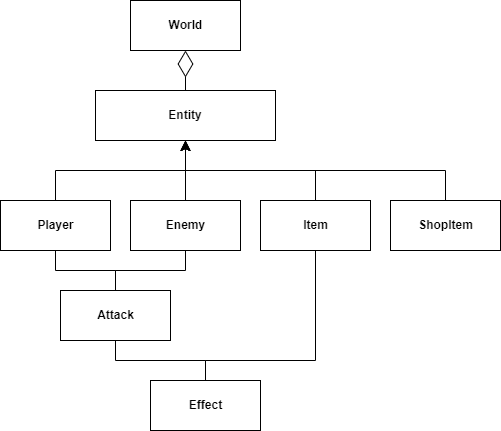
\includegraphics[width=\textwidth]{uml/img/uml_analisi_dominio.png}
	\caption{Diagramma uml concettuale rappresentante le varie entita' presenti nel dominio del gioco}
\end{figure}


\chapter{Design}


\section{Architettura}
Abbiamo deciso di utilizzare per il modello logico del gioco e per la logica di controllo una versione semplificata del pattern Entity-Component-System (ECS) mantenendo la parte grafica separata.
Questo pattern si basa come da definizione su tre parti fondamentali, che interconnesse permettono una buona suddivisione delle responsabilita', un alto riuso e un alto grado di composizione (composition over inheritance).



Di seguito spieghiamo le varie parti della nostra architettura:
\begin{itemize}
	\item Components: sono oggetti utili a mantenere dei dati che descrivono un certo aspetto del modello di gioco (ad esempio la posizione sul piano, il movimento ecc.). 
	\item Entity: sono dei raccoglitori di Component. Ogni entita' e' descritta dai suoi componenti che permettono alla stessa di distinguerla dalle altre entita'. Ad esempio, diverse entita' presenti in gioco nello stesso momento potrebbero contenere un PositionComponent, un MovementComponent, un BodyComponent, un HealthComponent e altri, che ne descrivono le proprieta' comuni. Tramite l'aggiunta di AIComponent o di un PlayerComponent, solo per citarne alcuni, e' possibile distinguere i nemici dal giocatore. 
	\item Systems: sono la parte dell'architettura che si occupa di operare sulle entita', modificandone i componenti e quindi svolgendo la maggior parte della logica del gioco. L'esecuzione sequenziale di vari sistemi, ciascuno che scorre le entita' e opera su un determinato set di componenti, permette il funzionamento del gioco. Ad esempio, il MovementSystem opera esclusivamente sulle entita' che contengono il MovementComponent e si occupa di muovere tutte le entita'; mentre il CheckHealthSystem si occupa di prendere tutte le entita' che hanno un HealthComponent e di rimuovere quelle che hanno esaurito le vite. E' quindi sufficiente, per inserire nel gioco una nuova meccanica, costruire nuovi componenti che definiscano nuove proprieta' e un nuovo sistema che operi su di essi senza il bisogno di andare a modificare i sistemi o i componenti precedentemente creati.
	\item Engine e World: queste sono le classi che controllano effettivamente lo svolgersi del gioco. Engine si occupa di gestire il game loop, mentre il World contiene al suo interno le entita' di gioco, schedula i system e passa alla View le informazioni necessarie.
	\item View: e' gestita in modo indipendente dal resto dell'architettura e si occupa solamente di disegnare lo stato del modello di gioco. Inoltre, gestisce diverse schermate, si occupa di disegnare l'interfaccia grafica e di registrare gli input da mouse e tastiera.
\end{itemize}

\pagebreak

\section{Design dettagliato}
\subsection{Lorenzo Prati}

\subsection{Elvis Perlika}

\subsection{Emanuele Dajko}

\subsection{Alessandra Versari}
\begin{itemize}
	\item Items: Con item si intende un oggetto di gioco che verrà raccolto a seguito del passaggio del player sopra ad esso. Gli item presenti nel nostro gioco sono cuori e monete.
	Ciascun item una volta entrato in contatto con un'entità deve prima verificare che si tratti del player ed effettuare i controlli necessari prima di applicare il proprio “effetto” (cioè la conseguenza/reazione che l'item avrà sull'entità che ha colliso con esso).
	Di seguito le principali caratteristiche degli items presenti nel nostro gioco:
	\begin{itemize}
		\item Gli items “cuore” permetteranno di aumentare la vita corrente del player, ma ciò verrà fatto solo a seguito del controllo sulla vita corrente: l'item verrà raccolto se e solo se la vita corrente è minore della vita massima che il player può avere. Questo tipo di item è disponibile in ogni stanza, escludendo lo Shop.
		\item Gli items “moneta”, anch'essi presenti in ciascun livello (shop escluso), permetteranno di aumentare l'ammontare delle monete raccolte dal player. Questo tipo di item, oltre a verificare che l'entità che ha colliso con esso sia il player, non farà ulteriori controlli. Lo scopo degli items “moneta” è quello di consentire al player, l'acquisto di power up (che tratterò in seguito) all'interno della stanza Shop.
	\end{itemize}
	Per realizzare quanto descritto ho deciso di creare due componenti principali: HealthComponent e CoinPocketComponent, appartenenti alla lista di componenti del player, che permettono di consultare e modificare vita corrente, vita massima e monete raccolte. Tramite i getter e i setter, in questo modo, posso creare gli “effetti” degli item, all'interno dell'ItemFactory. 
	Ogni item è dotato di un componente detto ItemComponent che oltre a rendere riconoscibili gli item, memorizza una Bifunction che corrisponde a quello che fin'ora ho definito “effetto”. La Bifunction in questo caso prende come argomento l'entità che ha colliso con l'item e una lista di component. Nel nostro gioco, al momento, solo il player ha la possibilità di raccogliere items, ma nel caso in cui volessimo rendere questi items raccoglibili anche ai nemici, sarebbe possibile farlo, passando come argomento alla Bifuntion una lista contenente i componenti identificativi di player e nemici (ossia PlayerComponent e AIComponent).
	Inizialmente avevo scelto di creare gli effetti utilizzando il Factory Method perché pensavo potesse rendere più riutilizzabili gli effetti e velocizzarne la creazione, ma il risultato era un insieme di classi Factory, molto simili tra loro e la cui unica differenza era operare su componenti diversi (una factory per gli effetti che modificavano la vita, un'altra per quelli che modificavano l'ammontare delle monete e così via).
	Inoltre siccome gli effetti alla fine sono praticamente solo incrementi e decrementi, mi è sembrato più sensato utilizzare interfacce funzionali e lamba per crearli all'interno della factory. 
	Per quanto riguarda le interfacce funzionali, ho deciso di utilizzare le Bifuction così da poter restituire un boolean che permette di capire se l'effetto è stato applicato o meno e se quindi è necessario rimuovere l'item.

	Nella classe ItemFactory è stato utilizzato il Factory Method.
	\item InteractableObjects: Con interactable objects si intende tutti gli oggetti di gioco che per essere utilizzati necessitano dell'interazione del giocatore. A differenza degli items infatti, la collisione con l'oggetto in questo caso non è sufficiente, è necessario premere in tasto E una volta posizionato il player sull'oggetto.
	Gli oggetti interactable presenti nel nostro gioco sono i power-up e il gate. 
	I power-up sono potenziamenti che il player può acquistare nella stanza shop pagando il loro prezzo. Essi si suddividono in:
	\begin{itemize} 
		\item Power-up vita: permette di aumentare la vita massima del giocare.
		\item Power-up velocità: permette di aumentare la velocità del giocatore.
	\end{itemize}
	Il gate invece è semplicemente il portale che permette di accedere al livello successivo. 
	Con gli items, anche gli interactable hanno degli “effetti” sul player e sul gioco stesso. 
	Il power-up vita infatti controlla che il player abbia monete sufficienti per eseguire l'acquisto, in caso affermativo viene modificato l'intero che indica la vita massima all'interno dell'HealthComponent.
	Il power-up velocità richiede anch'esso un controllo sulle monete raccolte dal giocatore e nel caso fossero sufficienti va ad aumentare il campo “speed” del MovementComponent.
	Il gate invece per poter essere attivato/utilizzato richiede che tutti i nemici siano stati eliminati e solo dopo aver fatto questo controllo lancerà l'evento ChangeRoomEvent() che permetterà di cambiare stanza.
	Una volta utilizzati, gli interactable objects vengono rimossi. 
	Per implementare tutto ciò ho utilizzato il Factory Method (vedi InteractableObjectFactory) per creare i vari oggetti interactable e ho implementato gli “effetti” di tali oggetti sempre all'interno della classe Interactablefactory (per gli stessi motivi degli items visti precedentemente). Per la creazione degli effetti ho utilizzato anche in questo caso interfacce funzionali (Bifunction, BiPredicate, Predicate e BiConsumer). 
	Oltre a necessitare l'interazione, questi oggetti si distinguono dagli items perché hanno la possibilità di lanciare eventi sul world all'interno del loro effetto.
	
	È stato utilizzato il Factory Method nella classe InteractableObjectFactory.
	\item Animazioni:
	\item Menù di gioco:
\end{itemize}



\subsection{Lorenzo Prati}

\subsubsection{Engine}

\begin{figure}[h]
	\centering
	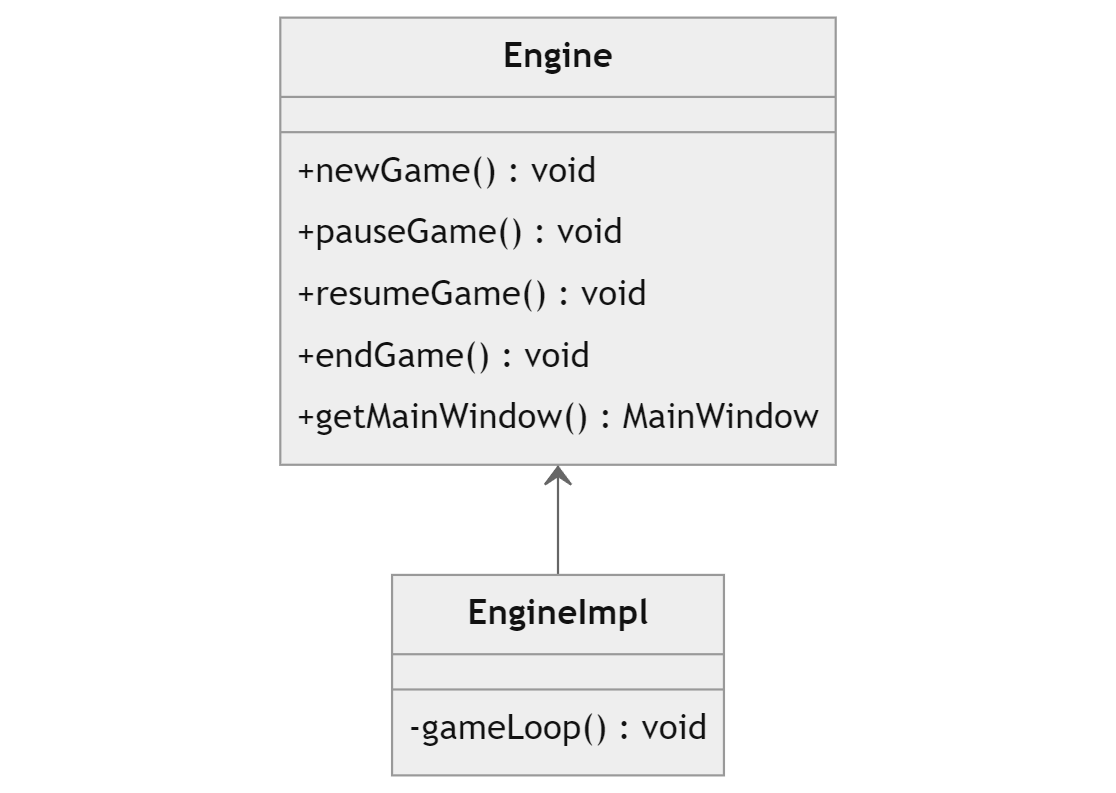
\includegraphics[width=\textwidth]{uml/uml_engine.png}
	\caption{Diagramma UML dell'Engine}
	\label{img:badarch}
\end{figure}

\paragraph*{Problema}
Realizzare una classe che permetta lo svolgimento effettivo del main loop del gioco, attraverso il quale scandire gli update del modello logico e della rappresentazione grafica, e che contenga tutti gli elementi per mantenere attiva l'applicazione. All'occorrenza, deve anche essere possibile mettere in pausa il gioco e riprenderlo. Deve essere inoltre gestita la fine del gioco.

\paragraph*{Soluzione} La soluzione e' ricaduta sulla creazione di un'interfaccia \texttt{Engine} con relativa implementazione \texttt{EngineImpl}. Questa classe fa uso del \textit{pattern game loop}, realizzato in un metodo privato e vengono esposti dall'interfaccia i metodi necessari alle altre classi (ad esempio le schermate della View) per controllare il loop. E' quindi possibile metterlo in pausa, riprenderlo e arrestarlo. Essendo questa classe la prima che viene creata al lancio dell'applicazione, essa si occupa anche internamente di creare il modello logico e la view.

\subsubsection{World}

\paragraph*{Problema}
Occorre contenere e mantenere il modello logico proprio del gioco, e comandare la logica che opera su di essi. Allo stesso tempo, e' necessario passare alla View le informazioni necessarie affinche' possa disegnare lo stato del dominio.

\paragraph*{Soluzione}
Ho scelto di unire in un'unica classe la funzione di contenere il dominio o modello logico, costituito di fatti dai dati contenuti nei \texttt{Component}, e la sua rappresentazione grafica (\texttt{Scene}), quindi ho realizzato l'interfaccia \texttt{World} con la relativa implementazone \texttt{WorldImpl}. Ho optato per questa scelta di nome nonostante la funzione della classe sia piu' comparabile a quella di un classico \textit{Controller} del pattern MVC poiche' e' utilizzato spesso nel contesto dell'ECS.

L'interfaccia \texttt{World} espone i metodi necessari al controllo del gioco vero e proprio, come ad esempio il metodo \textit{update}, che viene chiamato ad ogni ciclo \textit{game loop} in esecuzione sull'\texttt{Engine}. Questo e' il metodo principale della classe, perche' si occupa di:

\begin{itemize}
	\item eseguire tutti i \texttt{System}
	\item eseguire tutti gli eventi in coda nel \texttt{World}
	\item comandare alla scena di disegnare lo stato del gioco solo dopo aver passato le relative informazioni
\end{itemize}

Ho scelto di memorizzare e gestire i \texttt{System} direttamente in una lista dentro il \texttt{World} per semplicita' quando di fatti l'ordine con cui essi vengono memorizzati nella lista e quindi eseguiti ad ogni ciclo di \textit{update} potrebbe essere gestito da uno \textit{strategy pattern}; tuttavia ho scelto di semplificare l'approccio perche' in ogni caso non viene gestita in nessun modo l'abilitazione/disabilitazione di sistemi a run-time (come e' comune nel pattern ECS) e in generale in un gioco semplice come il nostro i pochi sistemi presenti devono eseguire strettamente uno dopo l'altro in un certo ordine preciso che di fatti lascia spazio a poche variazioni. Per quest'ultimo motivo, la gestione dei sistemi e' fissa e non modificabile, e per questo l'inizializzazione dei \texttt{System} e' gestita internamente al \texttt{World} e non e' visibile o modificabile dall'esterno.

Poi il \texttt{World} espone i metodi per la gestione delle \texttt{Entity}, cioe' che permettono di aggiungere e rimuovere \texttt{Entity}. 

Gli eventi sono gestiti tramite l'interfaccia \texttt{WorldEvent} e sono gestiti in modo asincrono. Durante la loro esecuzione, i vari \texttt{System} possono notificare il \texttt{World} di uno specifico evento, che verra' messo in una coda ed eseguito solo dopo che tutti i \texttt{System} hanno finito la loro esecuzione. In questo modo si evita il verificarsi di comportamenti anomali dovuti all'immissione di \texttt{Entity} nel \texttt{World} nel mezzo dei \texttt{System}. D'altra parte e' risultato comodo, durante l'esecuzione dei \texttt{System}, sia immettere che rimuovere le \texttt{Entity} tramite eventi dedicati, in modo da reagire all'aggiunta/eliminazione di una specifica entita' (ad esempio per il \textit{game over}). 

Inoltre, sono presenti vari metodi per settare e interrogare il risultato della partita, utili soprattutto all'\texttt{Engine} per stoppare il \textit{game loop}.


\chapter{Sviluppo}

\section{Testing automatizzato}

\section{Metodologia di lavoro}



\section{Note di sviluppo}



\chapter{Commenti finali}



\section{Autovalutazione e lavori futuri}



\section{Difficoltà incontrate e commenti per i docenti}



\appendix
\chapter{Guida utente}


\chapter{Esercitazioni di laboratorio}



\bibliographystyle{alpha}
\bibliography{13-template}

\end{document}
